\section{Результаты бенчмарков и сравнение версий}

\subsection{Влияние «эффекта наблюдателя» (Тестирование под leaks)}

При запуске тестов под утилитой проверки памяти \texttt{leaks} (с включенным \texttt{MallocStackLogging}) время работы программы значительно увеличивается. Это происходит из-за перехвата каждого вызова \texttt{new} для создания узлов дерева.

\begin{table}[h]
\centering
\small
\setlength{\tabcolsep}{6pt}  
\begin{tabular}{|l|c|c|c|}
\hline
\textbf{Алгоритм} & 
\textbf{Рекурсия} & 
\textbf{Итератив} & 
\textbf{Память (пик)} \\
\hline
\texttt{std::map} 
    & 790 ms & 820 ms & 296.2 MB \\
\hline
\textbf{avl::AVL} 
    & 1379 ms & \textbf{782 ms} & \textbf{299.7 MB} \\
\hline
Утечки 
    & 0 & 0 & — \\
\hline
\end{tabular}
\caption{Производительность и потребление памяти под \texttt{leaks} (643\,408 операций)}
\label{tab:leaks}
\end{table}

Несмотря на искажение времени, виден качественный скачок: итеративная версия требует почти в два раза меньше времени c этой утилитой.

\subsection{Нативные замеры производительности}

Для получения «чистых» метрик программа была скомпилирована с флагом \texttt{-O2} и запущена без инструментов отладки памяти.

\begin{table}[h]
\centering
\small
\setlength{\tabcolsep}{5pt}
\begin{tabular}{|l|c|c|c|c|}
\hline
\textbf{Алгоритм} 
    & \textbf{Время (рекурс.)} 
    & \textbf{Время (итерат.)} 
    & \textbf{RSS пик (рекурс.)} 
    & \textbf{RSS пик (итерат.)} \\
\hline
\texttt{std::map} (эталон) 
    & 507 ms & 502 ms & 250.2 MB & 250.2 MB \\
\hline
\texttt{avl::AVL} (наша реализация) 
    & 477 ms & \textbf{472 ms} & 248.5 MB & \textbf{247.4 MB} \\
\hline
\end{tabular}
\caption{Сравнение времени выполнения и пикового потребления памяти (RSS) при 643\,408 операциях}
\label{tab:memory}
\end{table}

Оптимизированная итеративная версия AVL-дерева оказалась быстрее \texttt{std::map} примерно на 5 миллисекунд на большом тесте по сравнению с рекурсивной.

\subsection{Анализ стека вызовов (Flame Graph)}

Для визуального анализа были построены **flame graphs** с помощью утилиты \texttt{samply} (или Xcode Instruments → Time Profiler).

\begin{figure}[h]
\centering
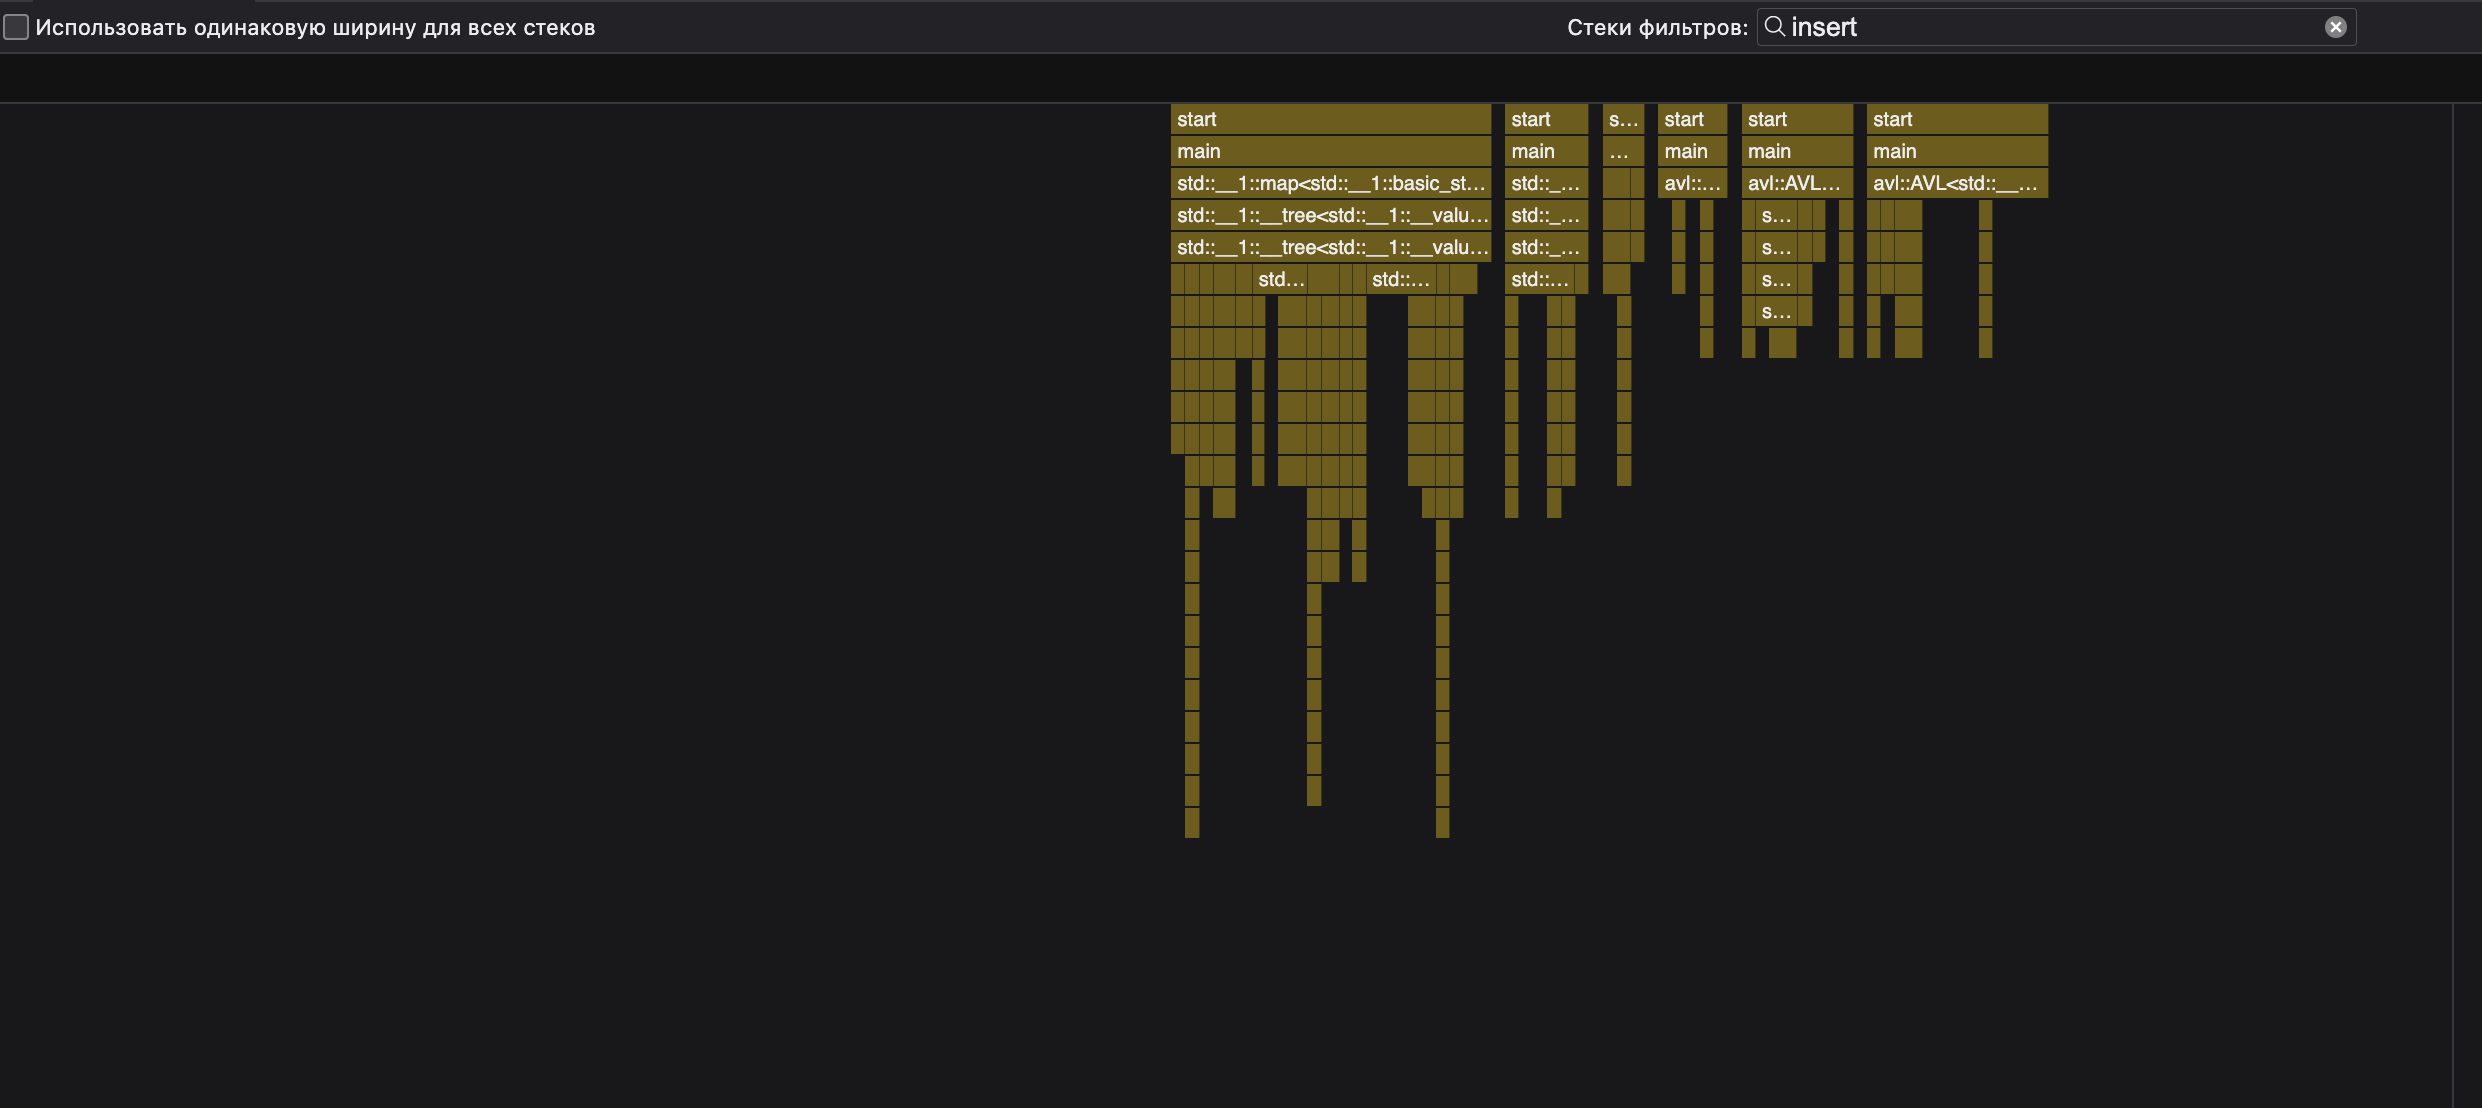
\includegraphics[width=0.95\linewidth]{img/iterative.png}
\caption{Flame Graph итеративной реализации insert (плоский стек вызовов)}
\end{figure}

\begin{figure}[h]
\centering
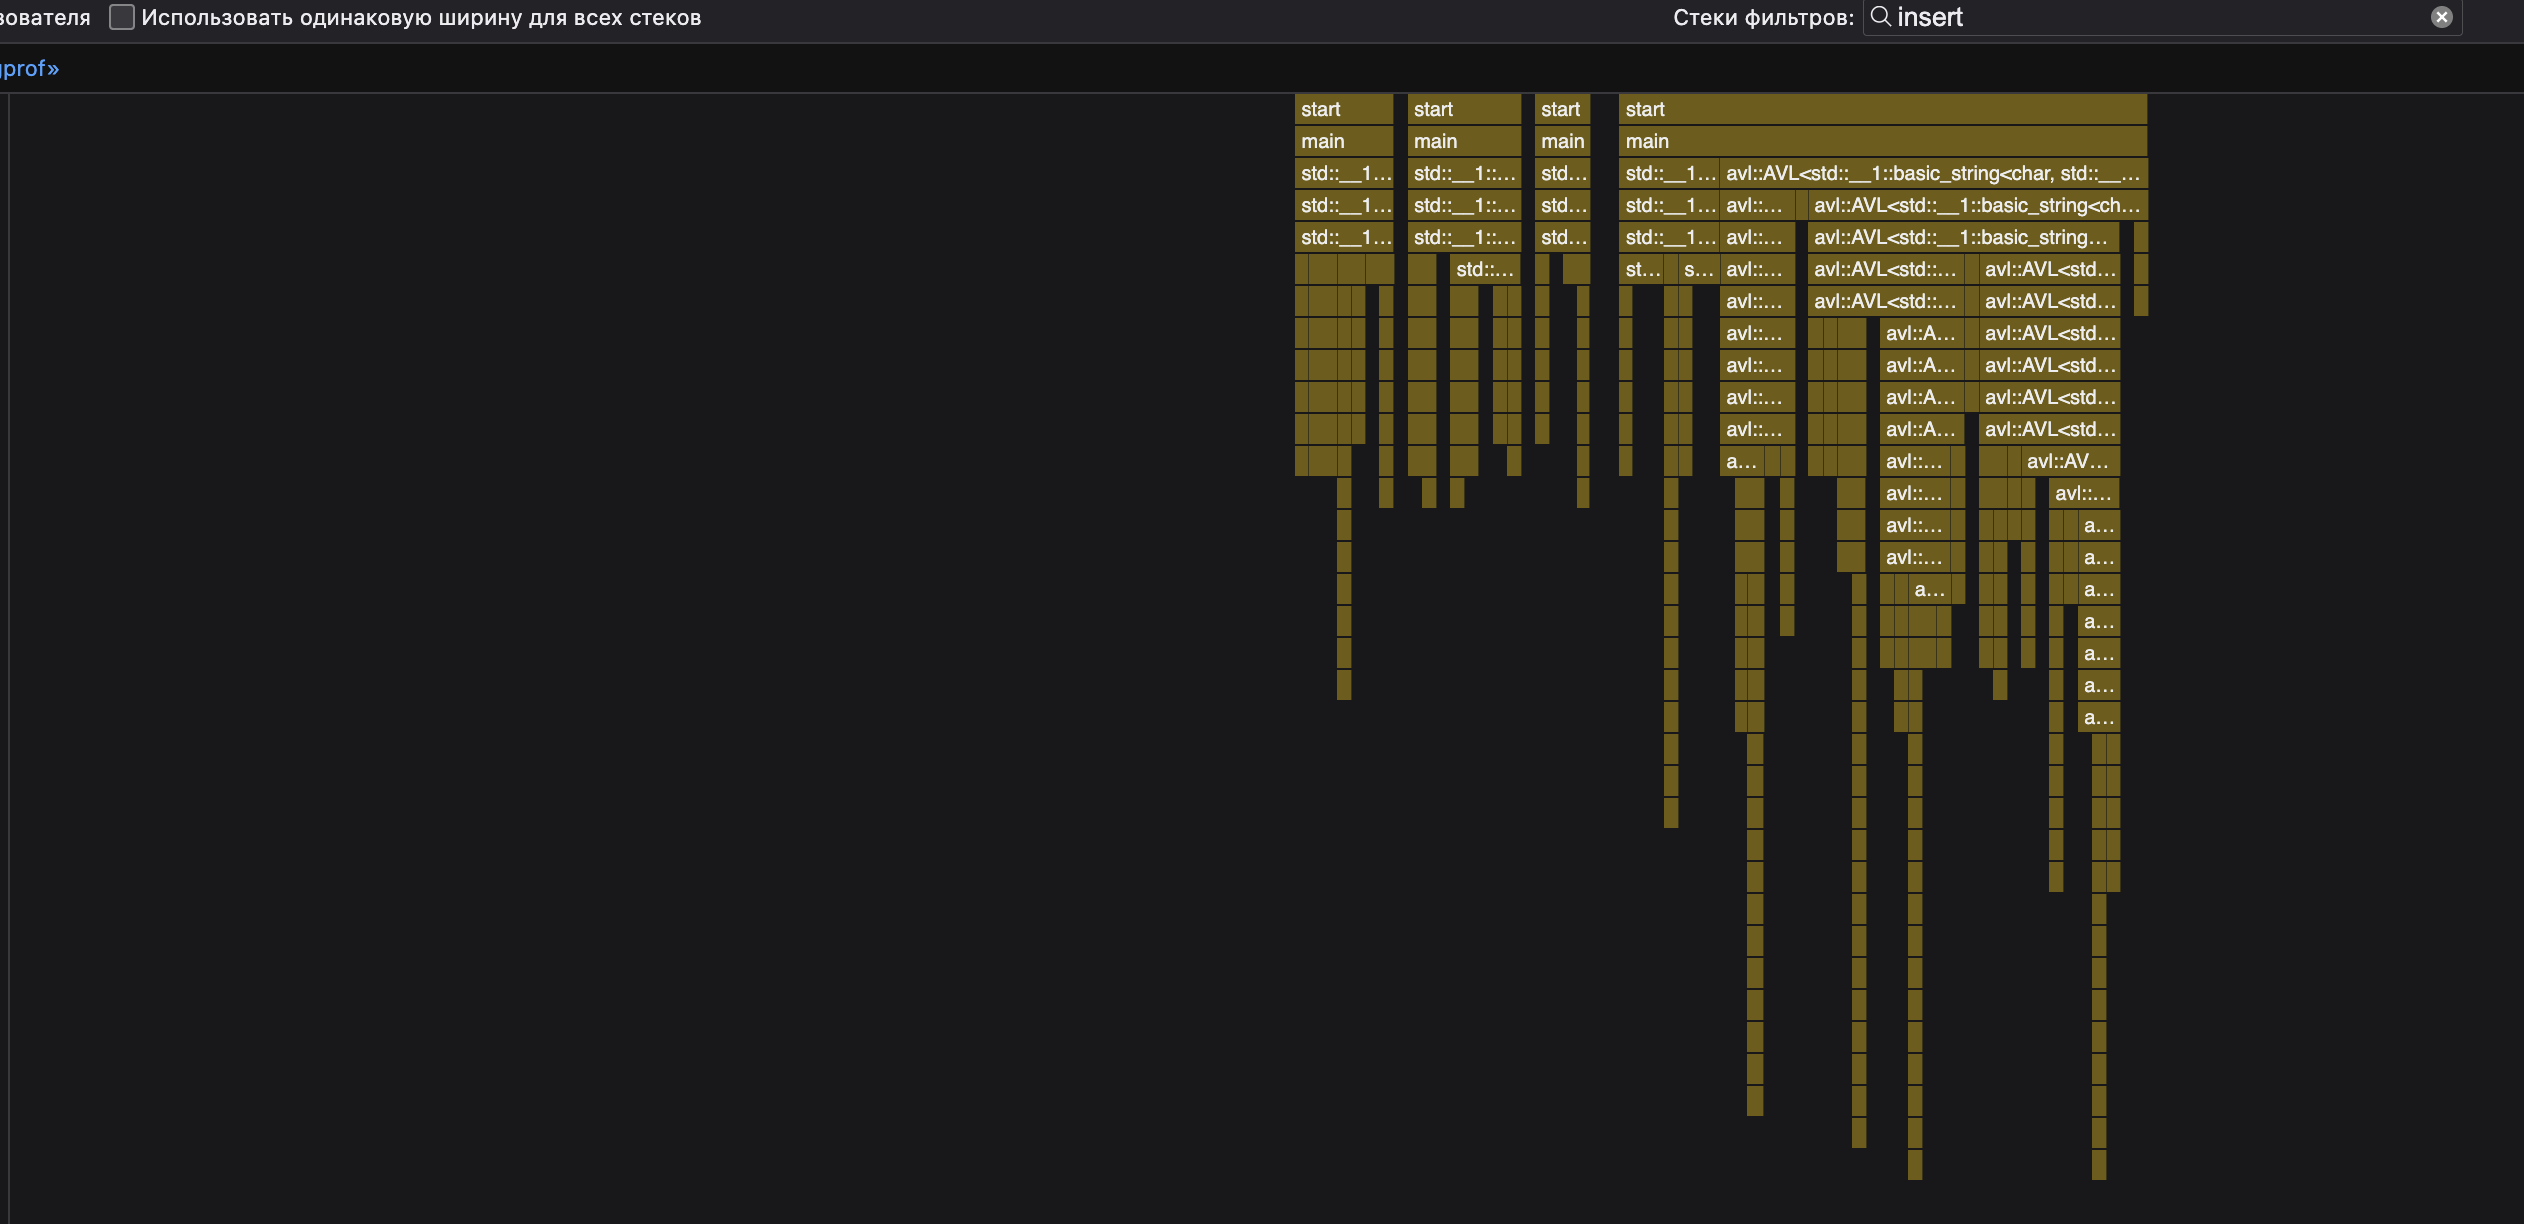
\includegraphics[width=0.95\linewidth]{img/recursive.png}
\caption{Flame Graph рекурсивной реализации insert (глубокая «лесенка» рекурсии)}
\end{figure}

На рекурсивной версии (Рис.~2) явно видна глубокая вложенность вызовов функции \texttt{insert} и \texttt{remove}. Итеративная версия (Рис.~1) имеет практически плоский профиль, который объясняется уходом от рекурсии.

\newpage